%% BioMed_Central_Tex_Template_v1.06
%%                                      %
%  bmc_article.tex            ver: 1.06 %
%                                       %

%%IMPORTANT: do not delete the first line of this template
%%It must be present to enable the BMC Submission system to
%%recognise this template!!

%%%%%%%%%%%%%%%%%%%%%%%%%%%%%%%%%%%%%%%%%
%%                                     %%
%%  LaTeX template for BioMed Central  %%
%%     journal article submissions     %%
%%                                     %%
%%          <8 June 2012>              %%
%%                                     %%
%%                                     %%
%%%%%%%%%%%%%%%%%%%%%%%%%%%%%%%%%%%%%%%%%

%%%%%%%%%%%%%%%%%%%%%%%%%%%%%%%%%%%%%%%%%%%%%%%%%%%%%%%%%%%%%%%%%%%%%
%%                                                                 %%
%% For instructions on how to fill out this Tex template           %%
%% document please refer to Readme.html and the instructions for   %%
%% authors page on the biomed central website                      %%
%% https://www.biomedcentral.com/getpublished                      %%
%%                                                                 %%
%% Please do not use \input{...} to include other tex files.       %%
%% Submit your LaTeX manuscript as one .tex document.              %%
%%                                                                 %%
%% All additional figures and files should be attached             %%
%% separately and not embedded in the \TeX\ document itself.       %%
%%                                                                 %%
%% BioMed Central currently use the MikTex distribution of         %%
%% TeX for Windows) of TeX and LaTeX.  This is available from      %%
%% https://miktex.org/                                             %%
%%                                                                 %%
%%%%%%%%%%%%%%%%%%%%%%%%%%%%%%%%%%%%%%%%%%%%%%%%%%%%%%%%%%%%%%%%%%%%%

%%% additional documentclass options:
%  [doublespacing]
%  [linenumbers]   - put the line numbers on margins

%%% loading packages, author definitions

%\documentclass[twocolumn]{bmcart}% uncomment this for twocolumn layout and comment line below
\documentclass{bmcart}

%%% Load packages
\usepackage{amsthm,amsmath}
%\RequirePackage[numbers]{natbib}
%\RequirePackage[authoryear]{natbib}% uncomment this for author-year bibliography
%\RequirePackage{hyperref}
\usepackage[utf8]{inputenc} %unicode support
%\usepackage[applemac]{inputenc} %applemac support if unicode package fails
%\usepackage[latin1]{inputenc} %UNIX support if unicode package fails


%%%%%%%%%%%%%%%%%%%%%%%%%%%%%%%%%%%%%%%%%%%%%%%%%
%%                                             %%
%%  If you wish to display your graphics for   %%
%%  your own use using includegraphic or       %%
%%  includegraphics, then comment out the      %%
%%  following two lines of code.               %%
%%  NB: These line *must* be included when     %%
%%  submitting to BMC.                         %%
%%  All figure files must be submitted as      %%
%%  separate graphics through the BMC          %%
%%  submission process, not included in the    %%
%%  submitted article.                         %%
%%                                             %%
%%%%%%%%%%%%%%%%%%%%%%%%%%%%%%%%%%%%%%%%%%%%%%%%%

\def\includegraphic{}
\def\includegraphics{}

%%% Put your definitions there:
\startlocaldefs
\endlocaldefs

%%% Begin ...
\begin{document}

%%% Start of article front matter
\begin{frontmatter}

\begin{fmbox}
\dochead{Research}

%%%%%%%%%%%%%%%%%%%%%%%%%%%%%%%%%%%%%%%%%%%%%%
%%                                          %%
%% Enter the title of your article here     %%
%%                                          %%
%%%%%%%%%%%%%%%%%%%%%%%%%%%%%%%%%%%%%%%%%%%%%%

\title{Prediction of Protein-Protein Interactions on the Human and Rice Interactomes}

%%%%%%%%%%%%%%%%%%%%%%%%%%%%%%%%%%%%%%%%%%%%%%
%%                                          %%
%% Enter the authors here                   %%
%%                                          %%
%% Specify information, if available,       %%
%% in the form:                             %%
%%   <key>={<id1>,<id2>}                    %%
%%   <key>=                                 %%
%% Comment or delete the keys which are     %%
%% not used. Repeat \author command as much %%
%% as required.                             %%
%%                                          %%
%%%%%%%%%%%%%%%%%%%%%%%%%%%%%%%%%%%%%%%%%%%%%%

\author[
  addressref={aff1},                   % id's of addresses, e.g. {aff1,aff2}
  corref={aff1},                       % id of corresponding address, if any
% noteref={n1},                        % id's of article notes, if any
  email={nicolaslopez@javerianacali.edu.co}   % email address
]{\inits{N.L.}\fnm{Nicolas A.} \snm{Lopez-Rozo}}
\author[
  addressref={aff1},
  email={jfinke@javerianacali.edu.co}
]{\inits{J.F.}\fnm{Jorge} \snm{Finke}}
\author[
  addressref={aff1},
  email={camilo.rocha@javerianacali.edu.co}
]{\inits{C.R.}\fnm{Camilo} \snm{Rocha}}

%%%%%%%%%%%%%%%%%%%%%%%%%%%%%%%%%%%%%%%%%%%%%%
%%                                          %%
%% Enter the authors' addresses here        %%
%%                                          %%
%% Repeat \address commands as much as      %%
%% required.                                %%
%%                                          %%
%%%%%%%%%%%%%%%%%%%%%%%%%%%%%%%%%%%%%%%%%%%%%%

\address[id=aff1]{%                           % unique id
  \orgdiv{Department of Electronics and Computer Science},             % department, if any
  \orgname{Pontificia Universidad Javeriana},          % university, etc
  \city{Cali},                              % city
  \cny{CO}                                    % country
}


%%%%%%%%%%%%%%%%%%%%%%%%%%%%%%%%%%%%%%%%%%%%%%
%%                                          %%
%% Enter short notes here                   %%
%%                                          %%
%% Short notes will be after addresses      %%
%% on first page.                           %%
%%                                          %%
%%%%%%%%%%%%%%%%%%%%%%%%%%%%%%%%%%%%%%%%%%%%%%

%\begin{artnotes}
%%\note{Sample of title note}     % note to the article
%\note[id=n1]{Equal contributor} % note, connected to author
%\end{artnotes}

\end{fmbox}% comment this for two column layout

%%%%%%%%%%%%%%%%%%%%%%%%%%%%%%%%%%%%%%%%%%%%%%%
%%                                           %%
%% The Abstract begins here                  %%
%%                                           %%
%% Please refer to the Instructions for      %%
%% authors on https://www.biomedcentral.com/ %%
%% and include the section headings          %%
%% accordingly for your article type.        %%
%%                                           %%
%%%%%%%%%%%%%%%%%%%%%%%%%%%%%%%%%%%%%%%%%%%%%%%

\begin{abstractbox}

\begin{abstract} % abstract

\parttitle{Background} %if any
Abstract A recent study in network-based prediction of protein-protein interactions (PPIs) reveals that two proteins are more likely to interact, the higher the number of paths of length 3 between them (normalized by the geometric average of their interactions). This paper extends previous work on mapping binary interactions by taking into account the learning of features (embeddings) of the PPI network. In particular, we implement a gradient boosted decision tree model (XGBoost) using handcrafted features (including the normalized measure) and embeddings from an algorithm that generates a low-dimensional representation of nodes (node2vec).

\parttitle{Results} %if any
Our main result shows that while the measure remains an important feature for predicting interactions, better performance is achieved when in addition embedding features are considered. The proposed approach is validated for the human and rice interactomes. For both cases, the combination of both types of features yield higher AUC values.

\parttitle{Conclusions} %if any
As found on this study on both human and rice, when information from handcrafted features based on neighborhood is enhanced with vector representations from random walks, the prediction power of the model improves. Besides, a supervised learning model can be trained for predicting unknown interactions based on such information. Finally, the developed framework can also be applied to interactomes of other organisms for which PPI networks have recently become available.

\end{abstract}

%%%%%%%%%%%%%%%%%%%%%%%%%%%%%%%%%%%%%%%%%%%%%%
%%                                          %%
%% The keywords begin here                  %%
%%                                          %%
%% Put each keyword in separate \kwd{}.     %%
%%                                          %%
%%%%%%%%%%%%%%%%%%%%%%%%%%%%%%%%%%%%%%%%%%%%%%

\begin{keyword}
\kwd{PPI}
\kwd{Prediction}
\kwd{Protein Interaction}
\kwd{Machine Learning}
\kwd{Python}
\kwd{XGBoost}
\kwd{node2vec}
\end{keyword}

% MSC classifications codes, if any
%\begin{keyword}[class=AMS]
%\kwd[Primary ]{}
%\kwd{}
%\kwd[; secondary ]{}
%\end{keyword}

\end{abstractbox}
%
%\end{fmbox}% uncomment this for two column layout

\end{frontmatter}

%%%%%%%%%%%%%%%%%%%%%%%%%%%%%%%%%%%%%%%%%%%%%%%%
%%                                            %%
%% The Main Body begins here                  %%
%%                                            %%
%% Please refer to the instructions for       %%
%% authors on:                                %%
%% https://www.biomedcentral.com/getpublished %%
%% and include the section headings           %%
%% accordingly for your article type.         %%
%%                                            %%
%% See the Results and Discussion section     %%
%% for details on how to create sub-sections  %%
%%                                            %%
%% use \cite{...} to cite references          %%
%%  \cite{koon} and                           %%
%%  \cite{oreg,khar,zvai,xjon,schn,pond}      %%
%%                                            %%
%%%%%%%%%%%%%%%%%%%%%%%%%%%%%%%%%%%%%%%%%%%%%%%%

%%%%%%%%%%%%%%%%%%%%%%%%% start of article main body
% <put your article body there>

%%%%%%%%%%%%%%%%
%% Background %%
%%
\section*{Introduction}

%Proteins are key actors of biological processes inside cells. Rather
than carrying out tasks as single agents, they are part of dynamic
networks of protein-protein interactions (PPI) \cite{Lin2017}. Such
networks underlie a variety of interdependent mechanisms, including
signal transduction, homeostasis control and stress responses. Furthermore,
PPI networks play an important role in physiological and developmental
processes such as protein phosphorylation, transcriptional co-factor
recruitment and transporter activation \cite{Zhang2010PPI}.

A common way to create PPI networks (or validate particular protein-protein
interactions) is the \emph{Yeast-Two-Hybrid} technique (also known
as \emph{two-hybrid screening} or \emph{Y2H}). Figure \ref{Y2H}A
illustrates the biological basis of Y2H: the expression of a specific
reporter gene is activated by the binding of a DNA-binding Domain
(DB) and an Activation Domain (AD) of a Transcription Factor, which
in turn binds to an Upstream Activation Sequence (UAS). To evaluate
an interaction between two proteins, the Y2H approach fuses one protein
to the DB domain (known as \emph{bait}) and another protein to the
AD (known as \emph{prey}). If the proteins interact, the reporter
gene expression is activated by the AD (Fig. \ref{Y2H}B). Otherwise,
if proteins fail to interact, the reporter gene is not expressed (Fig.
\ref{Y2H}C).

\begin{figure}[h]
\caption{\label{Y2H}The Yeast-2-Hybrid technique offers an experimental approach
for constructing PPI networks.}

%\noindent \centering{}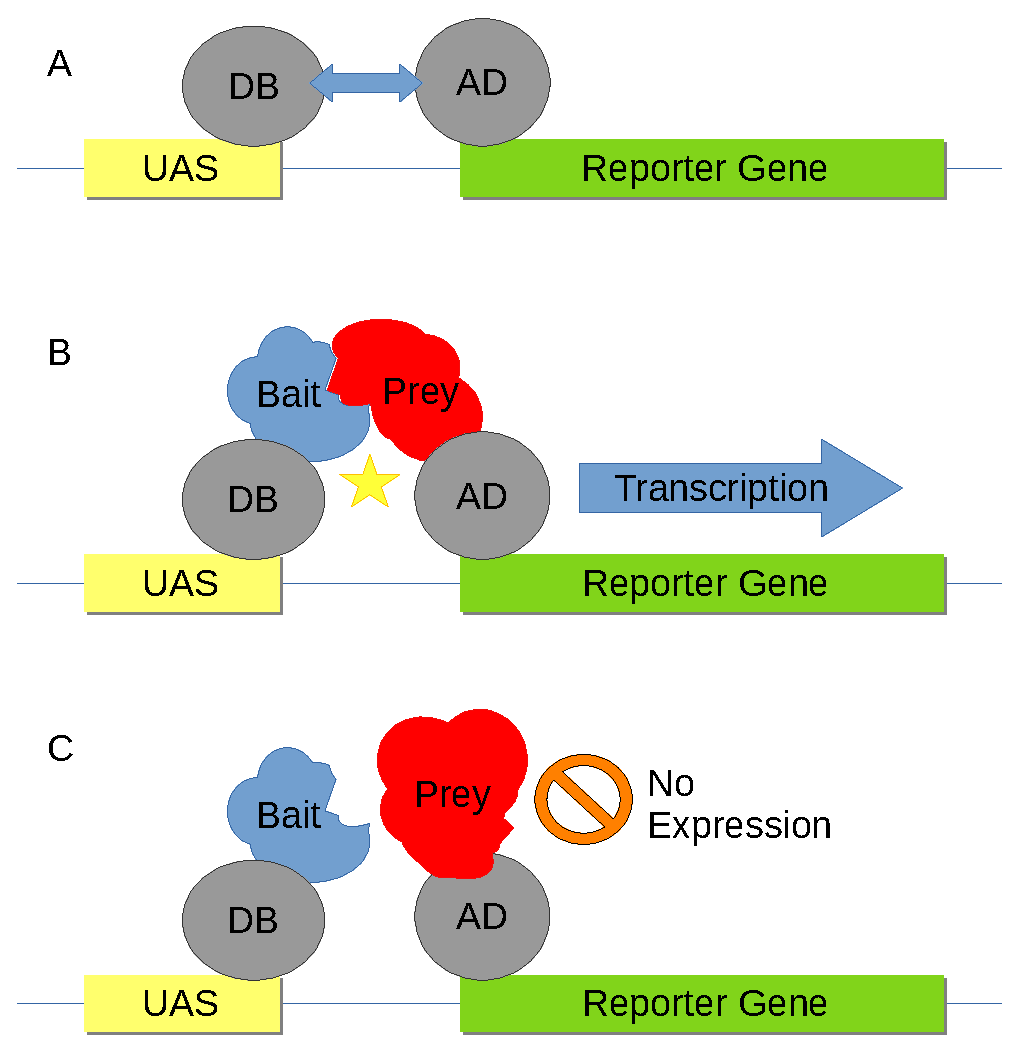
\includegraphics[width=0.7\columnwidth]{Y2H}
\end{figure}

Based on the outcome of numerous Y2H experiments, undirected networks
of interactions between proteins can be constructed. However, relying
only on experimental validation of PPIs is detrimental to research
due to its hindrance in costs, accuracy, required manpower and time
\cite{Laraia2015PPI,Macalino2018PPI}. Besides, the number of missing
interactions for pairs of proteins on many organisms leverage the
usage of computational methods for prediction of such interactions.

A common way of predicting interactions is usually based on social
networks analysis, more specifically on the triadic closure principle
(TCP). TCP states that the higher the number of common neighboring
nodes between two nodes, the higher the probability that they interact
\cite{Goldberg2003SmallWorld}. TCP can be addressed mathematically
by counting the number of shared neighbors of a pair of nodes, also
known as the Common Neighbors algorithm. By raising the adjacency
matrix (A) of the network to the second power (A\texttwosuperior ),
TCP can be considered for further analyses. However, previous studies
show that the mentioned approach usually fails because it does not
consider the structural and chemical properties of the proteins \cite{Cannistraci2013Networks,Kovacs2019}.

A variety of methods for predicting interactions in PPI networks have
been proposed in recent years \cite{Chang2016PPI,Chen2019PPI,Kotlyar2015PPI}.
Kovacs et al (2019) introduce a network-based approach which predicts
the interaction between two proteins based on the number of paths
of length 3, normalized by the geometric average of their interactions.
The simplest mathematical representation of this principle consists
on the third power of the adjacency matrix (A\textthreesuperior).
Furthermore, Kovacs et al present a degree-normalized scaling for
this metric, which reduces bias caused by intermediate hubs within
the paths of length 3. This handcrafted measure, denoted L3, enables
the proposed approach to outperform previous methods for predicting
binary protein interactions in yeast (\emph{S. cerevisiae}), Arabidopsis
(\emph{A. thaliana}), worm (\emph{C. elegans}), fly (\emph{D. melanogaster}),
fission yeast (\emph{S. pombe}), mouse (\emph{M. musculus}) and humans
\cite{Kovacs2019}.


The focus of this study is to evaluate different methods for predicting
PPIs using the network of known interactions. To achieve this, human
and rice PPI networks are compared using the proposed methods (A2,
A3, L3), as well as a low-dimensional representation of nodes (\texttt{Node2Vec})\cite{Grover_2016}.
After that, combinations of the two types of methods are tested. In
the case of the human network, two different versions of the human
interactome \cite{Rolland2014Human} are used for training and another
interactome version is used for validation (\emph{HI-III})\cite{Kovacs2019}.
For the rice interactome, a portion of the known interactions removed
and then predicted with different techniques based on the known interactions.
The main contributions of this paper are i) a general framework for
link prediction in non-directed networks and ii) two applications
of this framework to biological networks with a structural insight.

\paragraph*{Structure:} This paper is organized as follows. \emph{Materials and Methods} describes
the methodological steps and key milestones in the preparation of
the networks, model parameters and experimental configurations.
\emph{Results} presents the main results of the models for the human and rice interactomes.
\emph{Conclussions} presents the main conclusions of this study. Finally, \emph{Appendix}
presents supplementary information and figures which complement the
results described in this paper.

\subsection*{Sub-heading for section}
Text for this sub-heading\ldots
\subsubsection*{Sub-sub heading for section}
Text for this sub-sub-heading\ldots
\paragraph*{Sub-sub-sub heading for section}
Text for this sub-sub-sub-heading\ldots

In this section we examine the growth rate of the mean of $Z_0$, $Z_1$ and $Z_2$. In
addition, we examine a common modeling assumption and note the
importance of considering the tails of the extinction time $T_x$ in
studies of escape dynamics.
We will first consider the expected resistant population at $vT_x$ for
some $v>0$, (and temporarily assume $\alpha=0$)
%
\[
E \bigl[Z_1(vT_x) \bigr]=
\int_0^{v\wedge
1}Z_0(uT_x)
\exp (\lambda_1)\,du .
\]
%
If we assume that sensitive cells follow a deterministic decay
$Z_0(t)=xe^{\lambda_0 t}$ and approximate their extinction time as
$T_x\approx-\frac{1}{\lambda_0}\log x$, then we can heuristically
estimate the expected value as
%
\begin{equation}\label{eqexpmuts}
\begin{aligned}[b]
&      E\bigl[Z_1(vT_x)\bigr]\\
&\quad      = \frac{\mu}{r}\log x
\int_0^{v\wedge1}x^{1-u}x^{({\lambda_1}/{r})(v-u)}\,du .
\end{aligned}
\end{equation}
%
Thus we observe that this expected value is finite for all $v>0$ (also see \cite{koon,xjon,marg,schn,koha,issnic}).


\section*{Appendix}
Text for this section\ldots

%%%%%%%%%%%%%%%%%%%%%%%%%%%%%%%%%%%%%%%%%%%%%%
%%                                          %%
%% Backmatter begins here                   %%
%%                                          %%
%%%%%%%%%%%%%%%%%%%%%%%%%%%%%%%%%%%%%%%%%%%%%%

\begin{backmatter}

\section*{Acknowledgements}%% if any
Text for this section\ldots

\section*{Funding}%% if any
Text for this section\ldots

\section*{Abbreviations}%% if any
Text for this section\ldots

\section*{Availability of data and materials}%% if any
Text for this section\ldots

\section*{Ethics approval and consent to participate}%% if any
Text for this section\ldots

\section*{Competing interests}
The authors declare that they have no competing interests.

\section*{Consent for publication}%% if any
Text for this section\ldots

\section*{Authors' contributions}
Text for this section \ldots

\section*{Authors' information}%% if any
Text for this section\ldots

%%%%%%%%%%%%%%%%%%%%%%%%%%%%%%%%%%%%%%%%%%%%%%%%%%%%%%%%%%%%%
%%                  The Bibliography                       %%
%%                                                         %%
%%  Bmc_mathpys.bst  will be used to                       %%
%%  create a .BBL file for submission.                     %%
%%  After submission of the .TEX file,                     %%
%%  you will be prompted to submit your .BBL file.         %%
%%                                                         %%
%%                                                         %%
%%  Note that the displayed Bibliography will not          %%
%%  necessarily be rendered by Latex exactly as specified  %%
%%  in the online Instructions for Authors.                %%
%%                                                         %%
%%%%%%%%%%%%%%%%%%%%%%%%%%%%%%%%%%%%%%%%%%%%%%%%%%%%%%%%%%%%%

% if your bibliography is in bibtex format, use those commands:
\bibliographystyle{bmc-mathphys} % Style BST file (bmc-mathphys, vancouver, spbasic).
\bibliography{bmc_article}      % Bibliography file (usually '*.bib' )
% for author-year bibliography (bmc-mathphys or spbasic)
% a) write to bib file (bmc-mathphys only)
% @settings{label, options="nameyear"}
% b) uncomment next line
%\nocite{label}

% or include bibliography directly:
% \begin{thebibliography}
% \bibitem{b1}
% \end{thebibliography}

%%%%%%%%%%%%%%%%%%%%%%%%%%%%%%%%%%%
%%                               %%
%% Figures                       %%
%%                               %%
%% NB: this is for captions and  %%
%% Titles. All graphics must be  %%
%% submitted separately and NOT  %%
%% included in the Tex document  %%
%%                               %%
%%%%%%%%%%%%%%%%%%%%%%%%%%%%%%%%%%%

%%
%% Do not use \listoffigures as most will included as separate files

\section*{Figures}
  \begin{figure}[h!]
  \caption{Sample figure title}
\end{figure}

\begin{figure}[h!]
  \caption{Sample figure title}
\end{figure}

%%%%%%%%%%%%%%%%%%%%%%%%%%%%%%%%%%%
%%                               %%
%% Tables                        %%
%%                               %%
%%%%%%%%%%%%%%%%%%%%%%%%%%%%%%%%%%%

%% Use of \listoftables is discouraged.
%%
\section*{Tables}
\begin{table}[h!]
\caption{Sample table title. This is where the description of the table should go}
  \begin{tabular}{cccc}
    \hline
    & B1  &B2   & B3\\ \hline
    A1 & 0.1 & 0.2 & 0.3\\
    A2 & ... & ..  & .\\
    A3 & ..  & .   & .\\ \hline
  \end{tabular}
\end{table}

%%%%%%%%%%%%%%%%%%%%%%%%%%%%%%%%%%%
%%                               %%
%% Additional Files              %%
%%                               %%
%%%%%%%%%%%%%%%%%%%%%%%%%%%%%%%%%%%

\section*{Additional Files}
  \subsection*{Additional file 1 --- Sample additional file title}
    Additional file descriptions text (including details of how to
    view the file, if it is in a non-standard format or the file extension).  This might
    refer to a multi-page table or a figure.

  \subsection*{Additional file 2 --- Sample additional file title}
    Additional file descriptions text.

\end{backmatter}

\end{document}
